%!LW recipe=pdflatex

\documentclass[12pt,aspectratio=169]{beamer}
% \hypersetup{pdfpagemode=FullScreen}

\usepackage{upgreek}
\usefonttheme{professionalfonts}

\renewcommand*{\thefootnote}{\fnsymbol{footnote}}

\DeclareUnicodeCharacter{0301}{\'{e}}

\makeatletter
\def\onlyfootnote{\gdef\@thefnmark{}\@footnotetext}
\makeatother

\mode<presentation>
\useoutertheme[subsection=false]{miniframes}

\AtBeginSection[]{
    \begin{frame}
    \centering
    \begin{beamercolorbox}[sep=8pt,center,shadow=true,rounded=true]{title}
        \usebeamerfont{title}\insertsectionhead\par%
    \end{beamercolorbox}
    \end{frame}
}

\title{FlexGen: High-Throughput Generative Inference of Large Language Models with a Single GPU}
\author{ \small
    Ying~Sheng\inst{1}\and
    Lianmin~Zheng\inst{2}\and
    Binhang~Yuan\inst{3}\and
    Zhuohan~Li\inst{2}\and
    Max~Ryabinin\inst{4,5}\and
    Daniel~Y.~Fu\inst{1}\and
    Zhiqiang~Xie\inst{1}\and
    Beidi~Chen\inst{6,7}\and
    Clark~Barrett\inst{1}\and
    Joseph~E.~Gonzalez\inst{2}\and
    Percy~Liang\inst{1}\and
    Christopher~Ré\inst{1}\and
    Ion~Stoica\inst{2}\and
    Ce~Zhang\inst{3}
}
\institute{
    \inst{1}Stanford University \inst{2}UC Berkeley \inst{3}ETH Zurich \\
    \inst{4}Yandex \inst{5}HSE University \\
    \inst{6}Meta \inst{7}Carnegie Mellon University
}
\date{Presenter: Shiwei Zhang}

\begin{document}
    \beamertemplatenavigationsymbolsempty

    \begin{frame}
        \titlepage
    \end{frame}

    \section*{Content}

    \begin{frame}
        \frametitle{Content}

        \begin{itemize}
            \setlength{\itemsep}{.8em}
            \item Introduction
            \item Background: LLM Inference
            \item Offloading Strategy
            \item Approximate Methods
            \item Evaluation
            \item Conclusion
        \end{itemize}
    \end{frame}



    \section{Introduction}

    \begin{frame}
        \frametitle{Large Language Models}

        \begin{columns}
            \begin{column}{0.55\textwidth}
                Most of the state-of-the-art large language models use the decoder-only Transformer architecture.

                \vskip 1em
                They take a sequence of tokens as input and produce the probability distribution of the next token.
            \end{column}
            \begin{column}{0.45\textwidth}
                \vskip -1.5em
                \centering
                \includegraphics[page=3,trim=192.43bp 393.28bp 193.21bp 71.09bp,clip,scale=.65]{transformer.pdf}
            \end{column}
        \end{columns}
    \end{frame}

    \begin{frame}
        \frametitle{Interactive vs. Throughput-oriented Inference}

        \begin{columns}
            \begin{column}{0.5\textwidth}
                Interactive applications

                \vskip .5em
                \begin{itemize}
                    \setlength{\itemsep}{.5em}
                    \item Chat Bot
                    \item Customer Support
                    \item Search
                \end{itemize}
            \end{column}
            \begin{column}{0.5\textwidth}
                ``Back-of-house'' tasks are less sensitive to latency.

                \vskip .5em
                \begin{itemize}
                    \setlength{\itemsep}{.5em}
                    \item Information Extraction
                    \item Data Wrangling
                    \item Form Processing
                \end{itemize}
            \end{column}
        \end{columns}

        \vskip 2em
        It is possible to trade off latency for higher throughput in some workloads, providing opportunities to reduce
        resource requirements.
    \end{frame}

    \begin{frame}
        \frametitle{Latency-Throughput Trade-off}

        \centering
        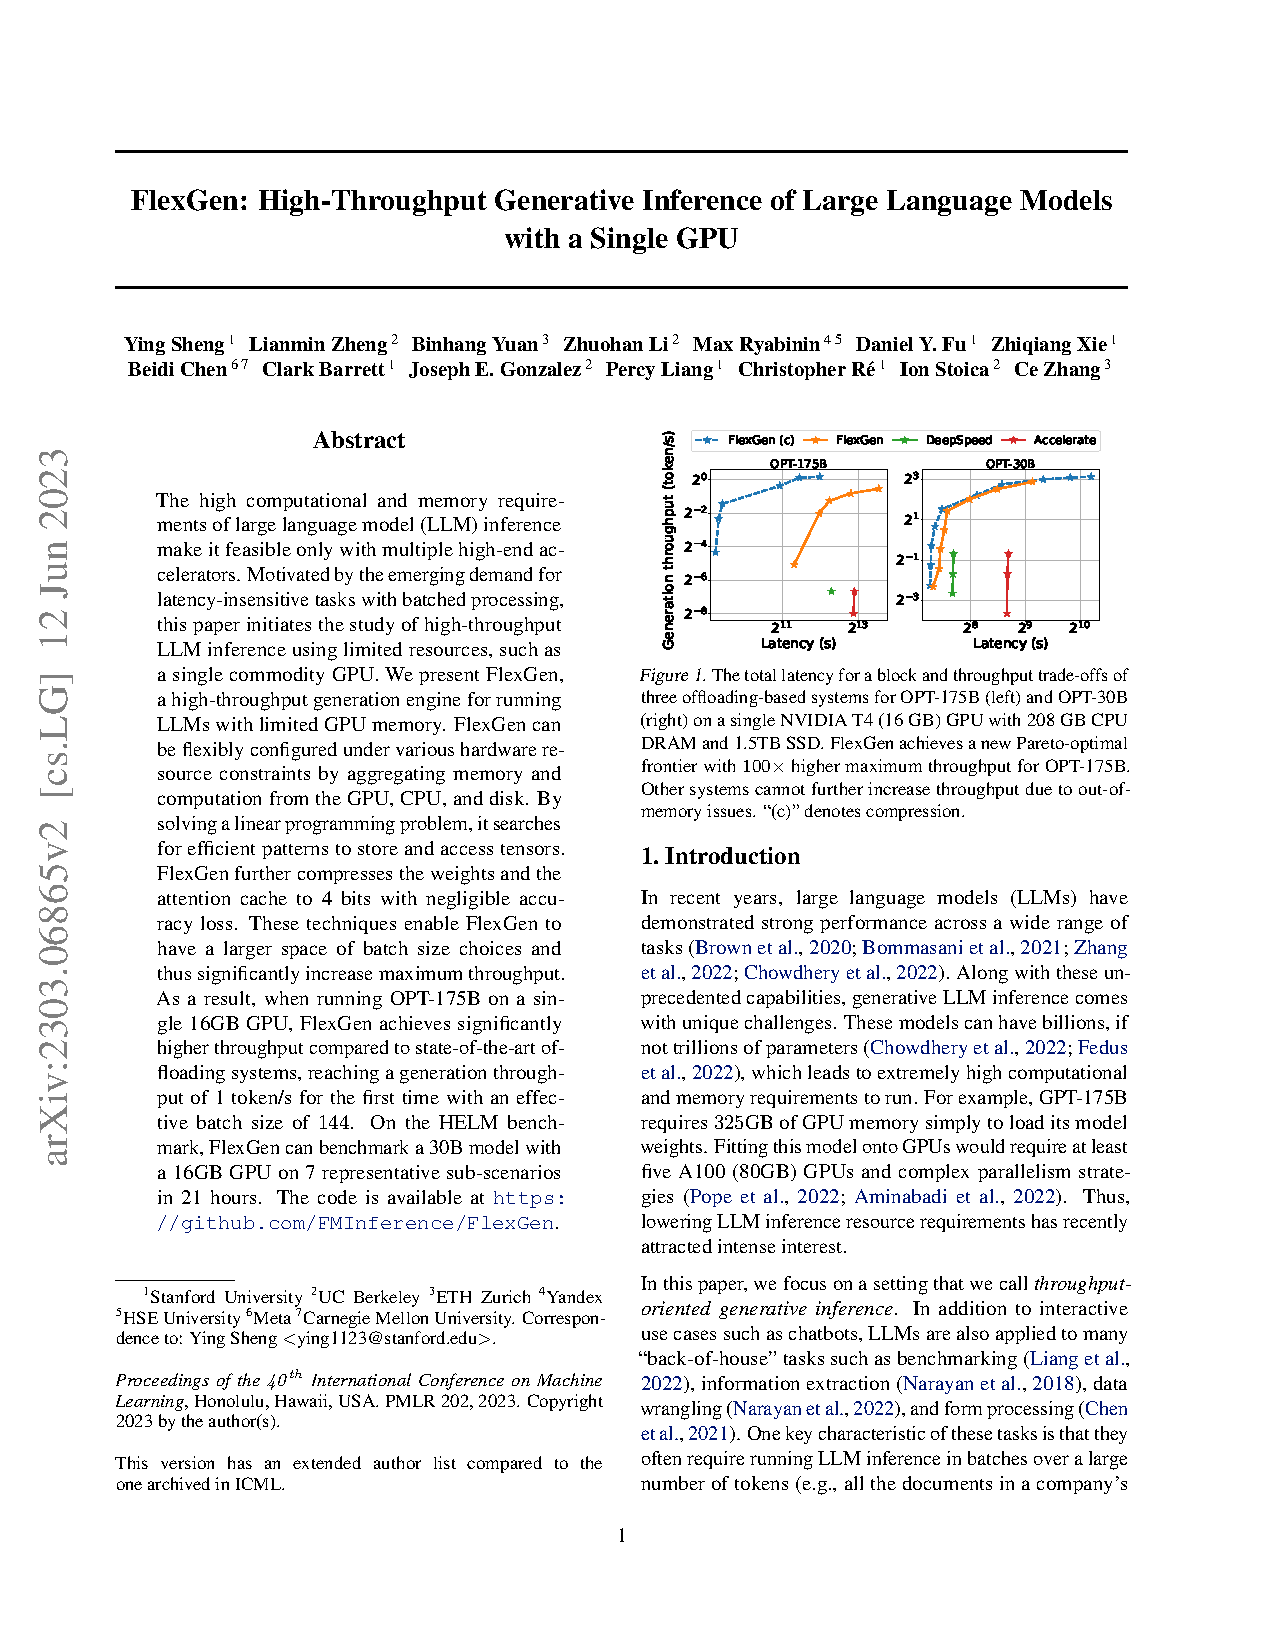
\includegraphics[page=1,trim=314.54bp 475.25bp 79.64bp 200.66bp,clip,scale=1.2]{paper.pdf}
    \end{frame}

    \begin{frame}
        \frametitle{Current State}

        \begin{itemize}
            \setlength{\itemsep}{.8em}
            \item FasterTransformer, Orca, LightSeq, PaLM, TurboTransformers, DeepSpeed Inference, and Hugging Face Accelerate focus on \textbf{latency-oriented} scenarios with \textbf{high-end accelerators}.
            \item DeepSpeed Inference and Hugging Face Accelerate supports offloading that is inherited from training systems. They fail to exploit the structure of the throughput-oriented LLM inference computation.
            \item Petals enable LLM inference on accessible hardware by collaborative computing.
        \end{itemize}
    \end{frame}

    \begin{frame}
        \frametitle{FlexGen}

        \begin{columns}
            \begin{column}{0.5\textwidth}
                The focus of this paper is designing efficient \textbf{offloading strategies} for high-throughput generative inference,
                on \textbf{a single commodity GPU}.
            \end{column}
            \begin{column}{0.5\textwidth}
                \centering
                \includegraphics[page=2,trim=207.56bp 368.48bp 319.13bp 353.49bp,clip,scale=1.2]{paper.pdf}
            \end{column}
        \end{columns}
    \end{frame}

    \begin{frame}
        \frametitle{Contributions}

        \begin{itemize}
            \setlength{\itemsep}{.8em}
            \item A strategy space considering computation schedule, tensor placement, and computation delegation.
            \item Compression of both the weights and KV cache without retraining or calibration.
            \item Experiments of OPT-175B on NVIDIA T4 (16GB) showing 100x/40x higher throughput with/without compression.
        \end{itemize}
    \end{frame}



    \section{Background: LLM Inference}

    \begin{frame}
        \frametitle{Generative Inference}

        A typical LLM generative inference task consists of two stages, the \textit{prefill stage} and the
        \textit{decoding stage}.

        \vskip 1em
        During the \textit{prefill phase}, the cached key and value vectors for each transformer layer is calculated.

        $$ \mathbf{x}_K^i = \mathbf{x}^i \cdot \mathbf{w}_K^i;\quad \mathbf{x}_V^i = \mathbf{x}^i \cdot \mathbf{w}_V^i;\quad \mathbf{x}_Q^i = \mathbf{x}^i \cdot \mathbf{w}_Q^i $$
        $$ \mathbf{x}_{Out}^i = \operatorname{Softmax}(\frac{\mathbf{x}_Q^i{\mathbf{x}_K^i}^T}{\sqrt{h}}) \cdot \mathbf{x}_V^i \cdot \mathbf{w}_O^i + \mathbf{x}^i $$
        $$ \mathbf{x}^{i+1} = \operatorname{relu}(\mathbf{x}_{Out}^i \cdot \mathbf{w}_1) \cdot \mathbf{w}_2 + \mathbf{x}_{Out}^i $$
    \end{frame}

    \begin{frame}
        \frametitle{Generative Inference (Cont'd)}

        During the \textit{decoding phase}, given $t^i$ as the embedding of the current generated token in the i-th
        layer:

        $$ \mathbf{x}_K^i \leftarrow \operatorname{Concat}(\mathbf{x}_K^i), \mathbf{t}^i \cdot \mathbf{w}_K^i;\quad \mathbf{x}_V^i \leftarrow \operatorname{Concat}(\mathbf{x}_V^i), \mathbf{t}^i \cdot \mathbf{w}_V^i;\quad \mathbf{t}_Q^i = \mathbf{t}^i \cdot \mathbf{w}_Q^i $$
        $$ \mathbf{t}_{Out}^i = \operatorname{Softmax}(\frac{\mathbf{t}_Q^i{\mathbf{x}_K^i}^T}{\sqrt{h}}) \cdot \mathbf{x}_V^i \cdot \mathbf{w}_O^i + \mathbf{t}^i $$
        $$ \mathbf{t}^{i+1} = \operatorname{relu}(\mathbf{t}_{Out}^i \cdot \mathbf{w}_1) \cdot \mathbf{w}_2 + \mathbf{t}_{Out}^i $$
    \end{frame}

    \begin{frame}
        \frametitle{Memory Analysis}

        Denote the batch size by $b$, the input sequence length by $s$, the output sequence length by $n$, the hidden
        dimensions of the Transformer and MLP layers by $h_1$ and $h_2$, and the number of layers by $l$.

        \vskip 1em
        The model weights is roughly (ignoring the embedding layer) $l(8h_1^2+4h_1h_2)$ bytes and the peak KV cache is $4blh_1(s+n)$.

        \vskip 1em
        The OPT-175B ($l=96$, $h_1=12288$, $h_2=49152$) model takes 325 GB. With $b=512$, $s=512$, and $n=32$, the KV
        cache is 1.2 TB, which is 3.8$\times$ the model weights.
    \end{frame}



    \section{Offloading Strategy}

    \begin{frame}
        \frametitle{Problem Formulation}

        The generative inference with offloading is formulated as a graph traversal problem. In the figure, a square
        means the computation of a GPU batch for a layer. The squares with the same color share the same layer weights.

        \vskip 1em
        \centering
        \includegraphics[page=4,trim=62.61bp 238.05bp 330.07bp 473.29bp,clip]{paper.pdf}
    \end{frame}

    \begin{frame}
        \frametitle{Problem Formulation (Cont'd)}

        A valid path is a path that traverses all squares under the following constraints:

        \vskip 1em
        \begin{itemize}
            \item A square can only be computed if all squares to its left on the same row were computed.
            \item To compute a square on a device, all its inputs must be loaded to the same device.
            \item After being computed, a square produces two outputs: activations and KV cache. The activations should
                  be stored until its right sibling is computed. The KV cache should be stored until the rightmost
                  square on the same row is computed.
            \item At any time, the total size of tensors stored on a device cannot exceed its memory capacity.
        \end{itemize}
    \end{frame}

    \begin{frame}
        \frametitle{Objective}

        The goal is to find a valid path that minimizes the total execution time, which includes the compute cost and
        I/O cost when moving tensors between devices.
    \end{frame}

    \begin{frame}
        \frametitle{Compute Schedule}

        All existing systems traverse the graph row-by-row to reduce latency.

        \vskip .5em
        \begin{center}
            \includegraphics[page=5,trim=63.60bp 569.75bp 331.12bp 67.54bp,clip,scale=.9]{paper.pdf}
        \end{center}

        The zig-zag block schedule reduces I/O costs by reusing the weights and KV cache for multiple batches. It
        introduces two parameters into the search space: the GPU batch size and the number of GPU batches in a block.
    \end{frame}

    \begin{frame}
        \frametitle{Compute Schedule with Overlapping}

        \begin{columns}
            \begin{column}{0.45\textwidth}
                Another typical optimization is overlapping the weights load of the next layer, cache/activation load of
                the next batch, cache/activation store of the previous batch, and the computation of the current batch.
            \end{column}
            \begin{column}{0.55\textwidth}
                \centering
                \includegraphics[page=5,trim=53.74bp 313.60bp 321.43bp 267.21bp,clip,scale=.85]{paper.pdf}
            \end{column}
        \end{columns}
    \end{frame}

    \begin{frame}
        \frametitle{Tensor Placement}

        FlexGen uses variables $wg$, $wc$, and $wd$ to define the percentages of \textbf{weights} stored on GPU, CPU,
        and disk, $hg$, $hc$, and $hd$ to define the percentages of \textbf{activations}, and $cg$, $cc$, $cd$ for the
        \textbf{KV cache}.

        \vskip 1em
        FlexGen uses layer granularity (e.g., assign 50\% of the tensors in a layer to the GPU) for weights, and tensor
        granularity (e.g., assign 50\% of the elements in a tensor to the GPU) for activations and the KV cache.
    \end{frame}

    \begin{frame}
        \frametitle{Computation Delegation}

        Using CPU for computation can be beneficial when the computation is I/O-bounded. Take the computation of
        attention scores $\operatorname{Softmax}(\frac{\mathbf{t}_Q^i{\mathbf{x}_K^i}^T}{\sqrt{h}})$ as example: the
        size of the moved KV cache is $b \times s \times h_1 \times 4$ bytes, and the size of the moved activation is $b
        \times h_1 \times 4$. For long sequences (e.g., $s \geq 512$), it is better to compute the attention scores on
        the CPU if the associated KV cache is not stored on the GPU.
    \end{frame}

    \begin{frame}
        \frametitle{Cost Model}

        The total latency for computing a block can be estimated as

        \vskip -.5em
        $$ T = T_{\text{pre}} \cdot l + T_{\text{gen}} \cdot (n - 1) \cdot l $$

        where $T_{\text{pre}}$ and $T_{\text{gen}}$ are the estimated latencies of the prefill stage and the decoding
        stage for one layer.
    \end{frame}

    \begin{frame}
        \frametitle{Cost Model (Cont'd)}

        Assuming perfect overlapping, $T_{\text{pre}}$ can be esitmated as

        \vskip -.5em
        $$ T_{\text{pre}} = \max(ctog^p, gtoc^p, dtoc^p, ctod^p, comp^p) $$

        where $ctog^p$, $gtoc^p$, $dtoc^p$, $ctod^p$, and $comp^p$ denote the latency of read from CPU to GPU, write
        from GPU to CPU, read from disk to CPU, write from CPU to disk, and computation, respectively, during prefill for
        one layer.

        \vskip 1em
        Similarly, $T_{\text{gen}}$ can be esitmated as

        \vskip -.5em
        $$ T_{\text{gen}} = \max(ctog^g, gtoc^g, dtoc^g, ctod^g, comp^g) $$

    \end{frame}

    \begin{frame}
        \frametitle{Cost Model Example}

        I/O terms like $dtoc^g$ are estimated by summing up the I/O events, which contain weights, activations, and
        cache reads.

        \vskip 1em
        The size of FP16 weights for one Transformer layer is $8h_1^2 + 4h_1 \cdot h_2$ bytes. Let $bls$ denote the block
        size and $s$ be the prompt length. The size of the activation for one layer is $2 \cdot bls \cdot h_1$ and the size of
        KV cache for one layer on average is $4 \cdot bls \cdot (s + \frac{n}{2}) \cdot h_1$.

        \vskip 1em
        Since $wd$, $hd$, and $cd$ percent of weights, activations, and KV cache are load from disk, the total latency
        of disk read is

        \vskip -1em
        $$ dtoc^g = \frac{1}{\text{bandwidth}}((8h_1^2 + 4h_1 \cdot h_2) \cdot wd + 2 \cdot bls \cdot h_1 \cdot hd + 4 \cdot bls \cdot (s + \frac{n}{2}) \cdot h_1 \cdot cd) $$
    \end{frame}

    \begin{frame}
        \frametitle{Policy Search}

        A policy includes 11 variables: block size $bls$, GPU batch size $gbs$, and 9 percentages for tensor placement.

        \vskip 1em
        FlexGen first enumerate a few choices of ($bls$, $gbs$) tuple. With fixed $bls$, $gbs$, the best placement
        becomes a linear programming problem.

        \vskip 1em
        \centering
        \includegraphics[page=6,trim=314.54bp 616.04bp 77.04bp 85.78bp,clip,scale=1.1]{paper.pdf}
    \end{frame}

    \begin{frame}
        \frametitle{Extension to Multiple GPUs}

        Tensor parallelism can reduce the single-query latency but pipeline parallelism can achieve good scaling on
        throughput due to its low communication costs.

        \vskip 1em
        FlexGen implements pipeline parallelism by equally partitioning an $l$-layer LLM on $m$ GPUs.
    \end{frame}



    \section{Approximate Methods}

    \begin{frame}
        \frametitle{Group-wise Quantization}

        FlexGen direclty quantize both the weights and KV cache into 4-bit integers without any retraining or
        calibration.

        \vskip 1em
        Given a tensor, FlexGen choose $g$ continous elements along a certain dimension as a group. For each group, the
        $min$ and $max$ are calculated and each element $x$ is quantized as

        $$ x_{\text{quant}} = \operatorname{round}(\frac{x - min}{max - min} \times (2^b - 1)) $$
    \end{frame}

    \begin{frame}
        \frametitle{Group-wise Quantization (Cont'd)}

        FlexGen uses 4 bits quantization with a group size of 64. The weights are grouped along the output channel
        dimension and the KV cache are grouped along the hidden dimension.

        \vskip 1em
        Fine-grained group-wise quantization in FlexGen causes some overhead in compression and decompression. Such an
        overhead could be very significant if run on a CPU which makes the CPU delegation useless, so FlexGen turns off
        the CPU delegation when enabling quantization.
    \end{frame}

    \begin{frame}
        \frametitle{Sparse Attention}

        After computing the attention matrices, for each query, FlexGen calculates the indices of the Top-K tokens from
        the K cache, then simply drops other tokens and only loads the subset of the V cache according to the indices.
    \end{frame}



    \section{Experiments}

    \begin{frame}
        \frametitle{Experimental Setup}

        \raisebox{3.5em}{\textbf{Hardware}:}
        \includegraphics[page=7,trim=325.88bp 663.67bp 91.10bp 74.45bp,clip,scale=.9]{paper.pdf}

        \vskip .5em
        \textbf{Models}: OPT models with 6.7B to 175B parameters.
        \vskip .5em
        \textbf{Workloads}: Synthetic datasets with all prompts padded to the 512/1024 tokens. The system is required to generate 32 tokens for each prompt.
        \vskip .5em
        \textbf{Implementation}: FlexGen is implemented on top of PyTorch. FlexGen manages multiple CUDA streams and CPU threads to overlap I/O with
        compute. FlexGen creates files for tensors stored on the disk and maps them as virtual memory to access them.
    \end{frame}

    \begin{frame}
        \frametitle{Baselines}

        \textbf{DeepSpeed Zero-Inference} supports offloading the whole weights to CPU or disk. It uses ZeRO data parallelism when given multiple GPUs.\\

        \vskip 1em
        \textbf{Hugging Face Accelerate} supports offloading a fraction of the weights.\\

        \vskip 1em
        \textbf{Petals} lowers the resource requirements for LLM inference with decentralized collaborative inference.\\
    \end{frame}

    \begin{frame}
        \frametitle{Maximum Throughput Benchmark}

        For OPT-175B, baseline systems can only use a GPU batch size of 2, but FlexGen can use a GPU batch size of 32
        and a block size of 32 $\times$ 8, achieving a 69$\times$ higher throughput

        \vskip 1em
        \centering
        \includegraphics[page=8,trim=309.19bp 535.82bp 71.96bp 168.37bp,clip,scale=1.1]{paper.pdf}
    \end{frame}

    \begin{frame}
        \frametitle{Maximum Throughput Benchmark with Multiple GPUs}

        FlexGen achieves super-linear scaling on decoding throughput with pipeline parallelism.

        \vskip 1em
        \centering
        \includegraphics[page=8,trim=308.91bp 409.75bp 71.69bp 323.38bp,clip,scale=1.1]{paper.pdf}
    \end{frame}

    \begin{frame}
        \frametitle{Latency-Throughput Trade-off}

        \centering
        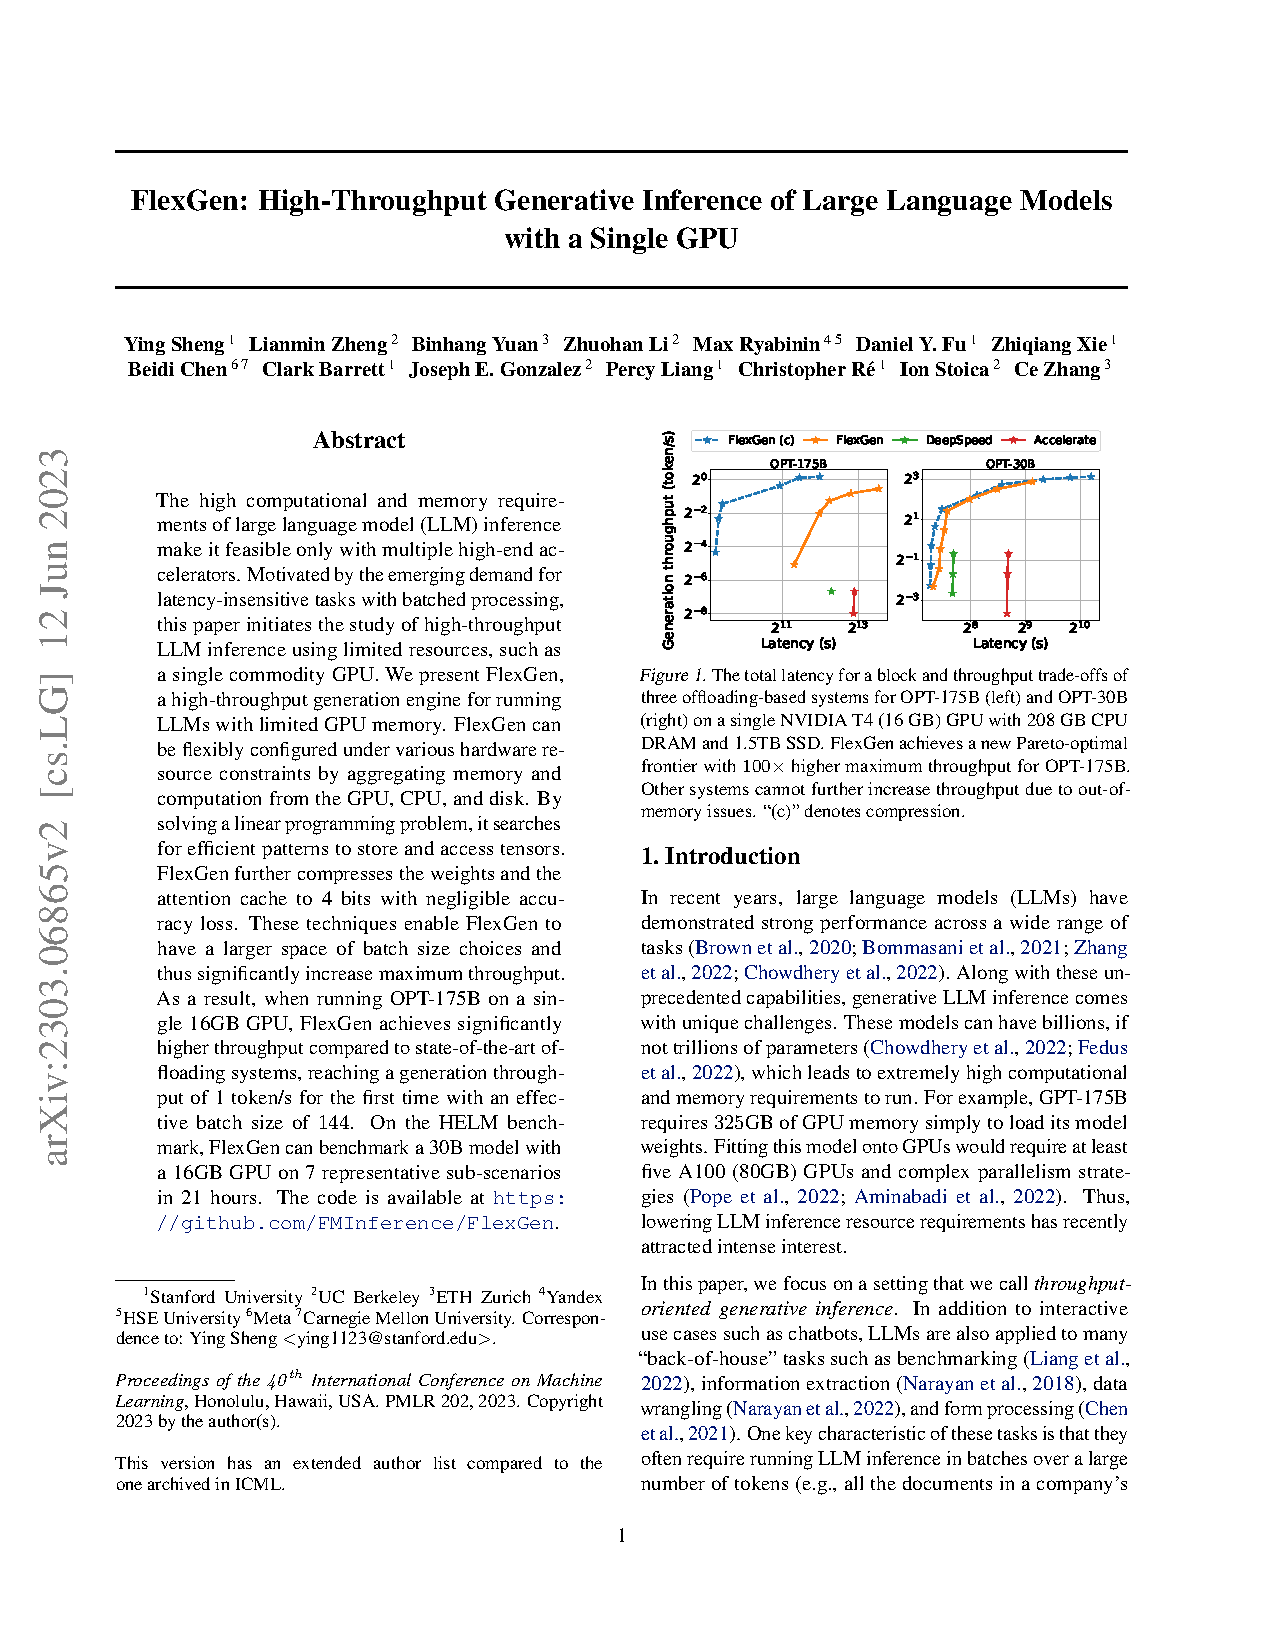
\includegraphics[page=1,trim=316.48bp 478.62bp 82.31bp 204.56bp,clip,scale=1.1]{paper.pdf}
    \end{frame}

    \begin{frame}
        \frametitle{Runtime Breakdown}

        \centering
        \includegraphics[page=18,trim=308.76bp 665.16bp 71.75bp 91.42bp,clip,scale=1.1]{paper.pdf}
    \end{frame}

    \begin{frame}
        \frametitle{Ablation Study}

        The numbers are generation throughput on 1 GPU with prompt length 512. The gray tuple denotes a policy (GPU
        batch size $\times$ \#GPU-batch, $wg$, $wc$).

        \vskip 1em
        \centering
        \includegraphics[page=9,trim=56.93bp 603.27bp 323.89bp 113.37bp,clip,scale=1.1]{paper.pdf}
    \end{frame}

    \begin{frame}
        \frametitle{Approximations}

        4-bit means using group-wise quantization to compress both weights and KV cache into 4-bit integers. 4-bit-S
        means combining the quantization and sparse attention with a 10\% sparsity on the value cache. Both methods show
        negligible accuracy loss compared to FP16.

        \vskip 1em
        \centering
        \includegraphics[page=9,trim=56.77bp 530.43bp 323.73bp 208.72bp,clip,scale=1.1]{paper.pdf}
    \end{frame}


    \begin{frame}
        \frametitle{Offloading vs. Collaborative Inference}

        The throughput of FlexGen with a single T4 outperforms the per-GPU throughput of the Petals cluster (4 nodes on
        GCP with one T4 GPU per node) under all tested network conditions.

        \vskip 1em
        \centering
        \includegraphics[page=9,trim=310.45bp 291.08bp 73.23bp 378.23bp,clip,scale=1.1]{paper.pdf}
    \end{frame}



    \section{Summary}

    \begin{frame}
        \frametitle{Strength}

        \begin{itemize}
            \setlength{\itemsep}{.8em}
            \item A new and important problem.
            \item In-depth analysis of the problem and locating the bottleneck with experiments.
            \item A lot of experiments (6 pages in the appendix).
        \end{itemize}
    \end{frame}

    \begin{frame}
        \frametitle{Limitation}

        \begin{itemize}
            \setlength{\itemsep}{.8em}
            \item The approximate methods are not novel and are not strongly related to other designs.
            \item The linear cost model does not reflect the fact that larger batch sizes bring better GPU utilization.
            \item The strategy space is not very complete and many of the decisions (e.g., CPU delegation) are manual.
            % \item The cost model assume perfect overlapping which is unrealistic.
        \end{itemize}
    \end{frame}

    \begin{frame}
        \frametitle{Takeaways}

        \begin{itemize}
            \setlength{\itemsep}{.8em}
            \item New scenarios (throughput-oriented LLM inference) brings new challenges to well-studied problems (offloading).
            \item It is easier to run experiments for resource-constraint systems.
            \item Search for parameters of well-designed heurstics instead of every possible solutions.\\
            ~~- It better illustrates the benefits instead of being pure ``black-box'' \\
            ~~- It may help maintain good performance with inaccurate profile data and imperfect cost models.
        \end{itemize}
    \end{frame}

    \appendix

    \begin{frame}
        \vskip 1em

        \centering \huge
        Thank you!
    \end{frame}
\end{document}
